\documentclass{beamer}
\usepackage[utf8]{inputenc}
\usepackage[english, russian]{babel}
\usepackage[T1, T2A]{fontenc}
\usepackage{tabu}
\setbeamertemplate{footline}[frame number]
\setbeamertemplate{headline}{}
\usepackage{graphicx}
\usepackage{color}
\usepackage{xcolor}
\usepackage{listings}
\definecolor{string}{HTML}{B40000} 
\definecolor{comment}{HTML}{008000} 
\definecolor{keyword}{HTML}{1A00FF} 
\definecolor{bk}{HTML}{FFFFFF} 
\definecolor{brackets}{HTML}{B40000}
\lstset{
	language=C++,
	keywordstyle=\color{keyword}\ttfamily\bfseries,
	stringstyle=\ttfamily\color{red!50!brown},
	commentstyle=\color{comment}\ttfamily, 
	breaklines=true, 
	breakatwhitespace=true, 
	basicstyle=\ttfamily\footnotesize, 
	backgroundcolor=\color{bk}, 
	tabsize=3,extendedchars=true,
	literate={а}{{\selectfont\char224}}1
	{б}{{\selectfont\char225}}1
	{в}{{\selectfont\char226}}1
	{г}{{\selectfont\char227}}1
	{д}{{\selectfont\char228}}1
	{е}{{\selectfont\char229}}1
	{ё}{{\"e}}1
	{ж}{{\selectfont\char230}}1
	{з}{{\selectfont\char231}}1
	{и}{{\selectfont\char232}}1
	{й}{{\selectfont\char233}}1
	{к}{{\selectfont\char234}}1
	{л}{{\selectfont\char235}}1
	{м}{{\selectfont\char236}}1
	{н}{{\selectfont\char237}}1
	{о}{{\selectfont\char238}}1
	{п}{{\selectfont\char239}}1
	{р}{{\selectfont\char240}}1
	{с}{{\selectfont\char241}}1
	{т}{{\selectfont\char242}}1
	{у}{{\selectfont\char243}}1
	{ф}{{\selectfont\char244}}1
	{х}{{\selectfont\char245}}1
	{ц}{{\selectfont\char246}}1
	{ч}{{\selectfont\char247}}1
	{ш}{{\selectfont\char248}}1
	{щ}{{\selectfont\char249}}1
	{ъ}{{\selectfont\char250}}1
	{ы}{{\selectfont\char251}}1
	{ь}{{\selectfont\char252}}1
	{э}{{\selectfont\char253}}1
	{ю}{{\selectfont\char254}}1
	{я}{{\selectfont\char255}}1
	{А}{{\selectfont\char192}}1
	{Б}{{\selectfont\char193}}1
	{В}{{\selectfont\char194}}1
	{Г}{{\selectfont\char195}}1
	{Д}{{\selectfont\char196}}1
	{Е}{{\selectfont\char197}}1
	{Ё}{{\"E}}1
	{Ж}{{\selectfont\char198}}1
	{З}{{\selectfont\char199}}1
	{И}{{\selectfont\char200}}1
	{Й}{{\selectfont\char201}}1
	{К}{{\selectfont\char202}}1
	{Л}{{\selectfont\char203}}1
	{М}{{\selectfont\char204}}1
	{Н}{{\selectfont\char205}}1
	{О}{{\selectfont\char206}}1
	{П}{{\selectfont\char207}}1
	{Р}{{\selectfont\char208}}1
	{С}{{\selectfont\char209}}1
	{Т}{{\selectfont\char210}}1
	{У}{{\selectfont\char211}}1
	{Ф}{{\selectfont\char212}}1
	{Х}{{\selectfont\char213}}1
	{Ц}{{\selectfont\char214}}1
	{Ч}{{\selectfont\char215}}1
	{Ш}{{\selectfont\char216}}1
	{Щ}{{\selectfont\char217}}1
	{Ъ}{{\selectfont\char218}}1
	{Ы}{{\selectfont\char219}}1
	{Ь}{{\selectfont\char220}}1
	{Э}{{\selectfont\char221}}1
	{Ю}{{\selectfont\char222}}1
	{Я}{{\selectfont\char223}}1
	{\{}{{{\color{brackets}\{}}}1 % Цвет скобок {
	{\}}{{{\color{brackets}\}}}}1 % Цвет скобок }
}
\setbeamertemplate{caption}[numbered]
\graphicspath{ {stepen'.png}{graf.png}{hromate.png}{raskraska.png}{g.png}{g1.png}{g2.png}{g3.png}{Greedy.png}{kod.png}{polnyi.png}{polnyi1.png}{color_tabl.png}{start.jpg}{massive.jpg}{end.jpg}{polnyiper.png}{polnyiper1.png}{polnyiper2.png}{polnyiper3.png}{polnyiper4.png}}

\title{Раскраска графа}
\author{Шамакова Екатерина}
\institute{shamaich0168@gmail.com}
\thispagestyle{empty}
\date{}

\begin{document}

	\frame {
		\titlepage
	}
	
	\frame {
		\frametitle{План:}
		\begin{itemize}
			\item Что такое граф и основные определения, связанные с ним
			\item Постановка задачи
			\item Алгоритмы реализации раскаски графа
			\begin{itemize}
				\item Полный перебор
				\item Жадный алгоритм
			\end{itemize}
			\item Инструкция пользователя
			\item Выводы
		\end{itemize}
	}
	
	\frame{
		\frametitle{Основные определения}
		Графом называют математическую модель, представляющую собой множество вершин и набор рёбер

		Вершины: { 1, 2, 3, 4, 5, 6, 7, 8}

		Рёбра: 1-2,	 1-5,	 2-3,	 3-4,	 5-4	  ...
		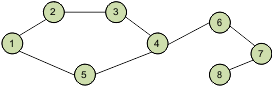
\includegraphics{graf} 

		Две вершины считаются \textbf{\textit{смежными}}, если имеют хотя бы одно общее ребро
	 }
	 
	\frame{
		\frametitle{Основные определения}
		 \begin{figure}
			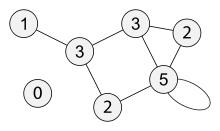
\includegraphics{stepen'}
			\caption{Граф, на вершинах которого отмечены степени}
		\end{figure}

		\textbf{\textit{Степень}} или \textbf{\textit{валентность}} вершины графа — это число ребер, входящих в эту вершину. 
	}
		
	\frame{
	 	\frametitle{Основные определения}
		Наименьшее число красок, необходимое для правильной раскраски графа G называется\textbf{\textit{хроматическим числом}}  графа G. Хроматическое число обозначается через $\chi(G)$.
		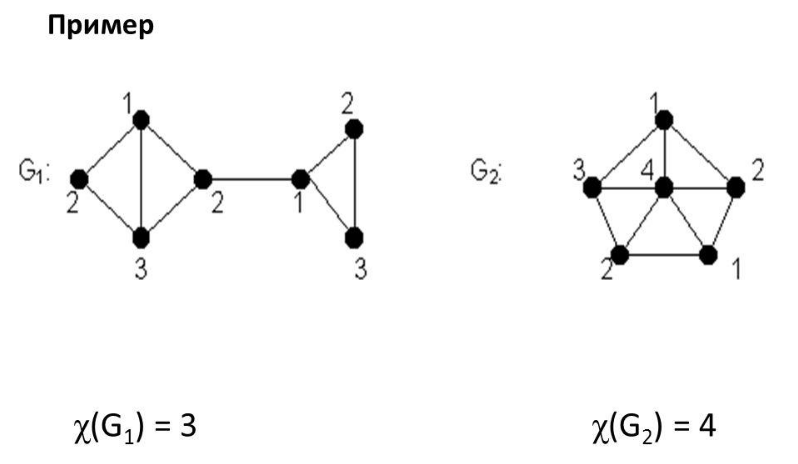
\includegraphics[scale=0.5]{hromate}

	}
	
	\frame{
		 \frametitle{Раскраска графа}
		 \begin{itemize}
			\item Раскрасить вершины графа
			\item Любые 2 смежные вершины имеют разные цвета
			\item Используя минимальное количество цветов
		\end{itemize}
		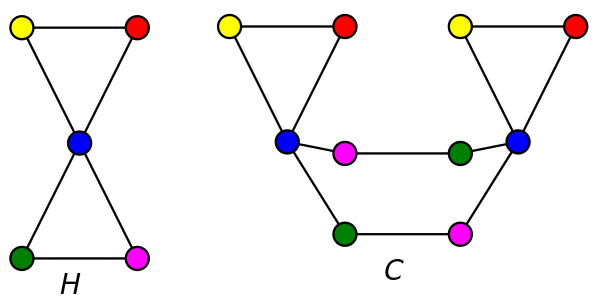
\includegraphics[scale=0.5]{raskraska}

	}
		
	\frame{
		\frametitle{Алгоритмы раскраски графа}
		\begin{itemize}
			\item Полный перебор
			\item Жадный алгоритм
		\end{itemize}
	}
	
	\frame{
		\frametitle{Алгоритмы раскраски графа}
		Способ хранения раскрашенных вершин: vector< list< int > > table


		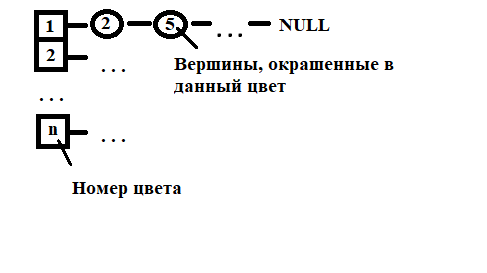
\includegraphics[scale=0.8]{color_tabl}
	}
		
	\frame{
		 \frametitle{Полный Перебор}
		Пробуем раскрасить граф, последовательно увеличивая количество цветов, начиная с 1, пока не останется нераскрашенных вершин. То число цветов, которым получится раскрасить граф, и будет его хроматическим числом.


		\begin{figure}
			\centering
			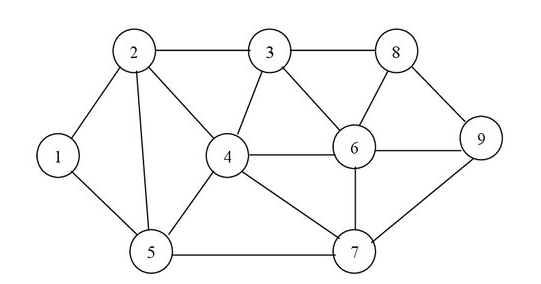
\includegraphics[scale=0.5]{polnyiper}
			\caption{Начальный граф}
		\end{figure}
	}
	
	\frame{
	 	\frametitle{Этапы работы полного перебора}
	 	\begin{figure}[!tbp]
	 		\centering
		 	\begin{minipage}[b]{0.4\textwidth}
				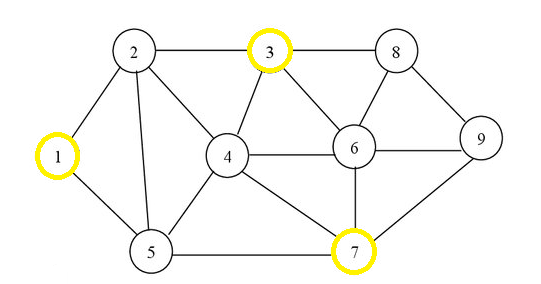
\includegraphics[width=\textwidth]{polnyiper1}
				\caption{Раскрашиваем его 1 цветом}
			\end{minipage}
			\hfill
			\begin{minipage}[b]{0.4\textwidth}
				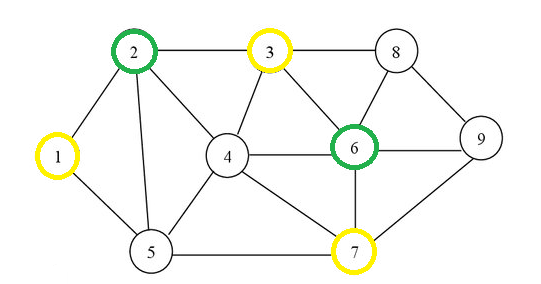
\includegraphics[width=\textwidth]{polnyiper2}
				\caption{Раскрашиваем его 2 цветами}
			\end{minipage}
			\hfill
			\begin{minipage}[b]{0.4\textwidth}
				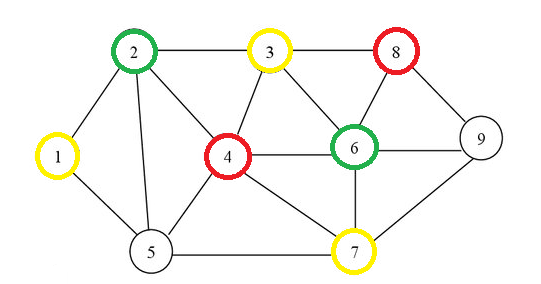
\includegraphics[width=\textwidth]{polnyiper3}
				\caption{Раскрашиваем его 3 цветами}
			\end{minipage}
			\hfill
			\begin{minipage}[b]{0.4\textwidth}
				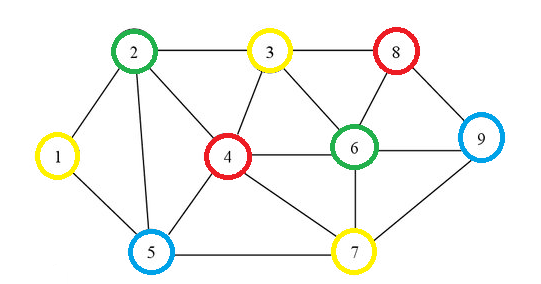
\includegraphics[width=\textwidth]{polnyiper4}
				\caption{Раскрашенный граф}
			\end{minipage}
		\end{figure}
		
	}
	
	\begin{frame}[fragile]
		\frametitle{Полный перебор (псевдокод)}
		Вызов из main\\
		\begin{lstlisting}
   
 int main()
{
	...
    bool done=false;  //проверка, все ли вершины смогли окрасить
    int max_color=1;
    while(done!=true){ //пока остались нераскрашенные вершины
    done=brute_fofce(0, max_color);
    max_color++;	//увеличиваем число красок
   	...
}
		\end{lstlisting}
	\end{frame}
	
	\begin{frame}[fragile]
		\frametitle{Полный перебор (псевдокод)}
		\begin{lstlisting}
bool brute_force(int k, int max_color) {
	if(все вершины окрашены)
	{
		chromatic_number = max_color;
		return true;
	}
	else {
		for (от минимального цвета до максимального) {
			for (по списку вершин с одним цветом)
				//если не смежна ни с одной из них
				//раскрашиваем вершину																	brute_force(k + 1, max_color);
				if (окрасили последнюю вершину)
					//переходим к концу функции
				else
					//удаляем цвет
		}
	}
}

	\end{lstlisting}
	\end{frame}
		
	\frame{
		\frametitle{Жадный алгоритм}
		\begin{enumerate}
			\item Сортируем вершины по их степеням в порядке убывания.
			\item  Последовательно окрашиваем вершины в выбранный цвет. Если у вершины уже есть смежная вершины с выбранный цветом, то оставляем ее неокрашенной.
			\item Если остались неокрашенные вершины, то выбираем следующий цвет и возвращемся ко 2 пункту.
		\end{enumerate}

		Качество полученной раскраски зависит от выбранного порядка.Жадный не всегда даёт оптимальное решение.

		Например:
		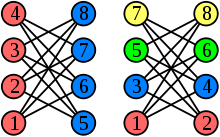
\includegraphics[scale=0.5]{Greedy}

	}
		
	\frame{
		\frametitle{Этапы работы жадного алгоритма}
		\begin{figure}[!tbp]
			 \centering
			 \begin{minipage}[b]{0.4\textwidth}
				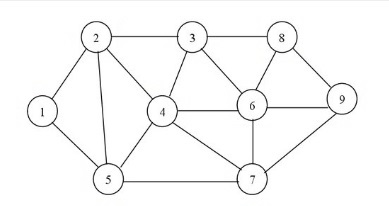
\includegraphics[width=\textwidth]{start}
				\caption{Граф до работы алгоритма}
			\end{minipage}
			\hfill
			\begin{minipage}[b]{0.4\textwidth}
				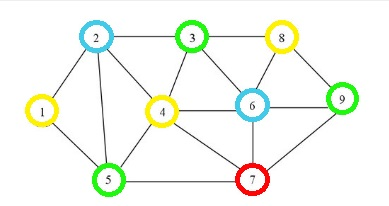
\includegraphics[width=\textwidth]{end}
				\caption{Раскрашенный граф}
			\end{minipage}
			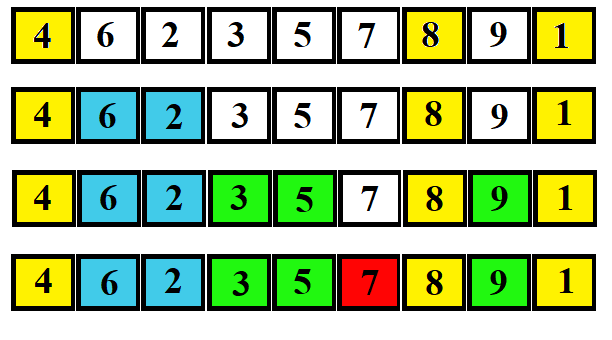
\includegraphics[scale=0.4]{massive}
			\caption{этапы работы жадного алгоритма}
		\end{figure}		
	}
		
	
	\begin{frame}[fragile]
		\frametitle{Жадный алгоритм (псевдокод)}
		\begin{lstlisting}
vector< list <int> > greedy() {
	//сортируем вершины графа в порядке убывания их степеней
	for (по всем вершинам) {
		if (вершина не раскрашена) {
			//добавляем её в список (присваиваем ей цвет)
			for (int j = i + 1; j < size; j++) {
				if (вершина не окрашена) {
					for (по списку вершин, принадлежащих одному цвету) {
					//если не смежна ни с одной из вершин
					//раскрашиваем её
					}
				}
			}
			//переходим к следующему цвету
		}
	}
}

	\end{lstlisting}
	\end{frame}
	
	\frame{
		\frametitle{Инструкция пользователя}
		Необходимо ввести: in.txt out.gv algNum
		\begin{itemize}
			\item in.txt: текстовый файл, в котором первой строкой записано количество вершин графа, а далее -- матрица смежности через пробел
			\item out.gv: файл, в который запишется раскрашенный граф в формате graphviz
			\item algNum: 0-полный перебор, 1-жадный алгоритм
		\end{itemize}

		Пример файла in.txt:

		3

		\begin{tabular}{c c c }
			0 & 1 & 1 \\
			1 & 0 & 1 \\
			1 & 1 & 0
		\end{tabular}

		Далее в ходе выполнения программы необходимо будет ввести указанное количество цветов на английском языке через "Enter"
	}
	
	\frame{
	 	\frametitle{Вывод}
		\begin{center}
			\begin{tabu} to 1.0\textwidth { | X[l] | X[c] | X[r] | }
 				\hline
			 	Название алгоритма & Сложность & Качество \\
				\hline
				Жадный алгоритм  &  О(\(n^3\)) & есть контр. пример  \\
				\hline
				Полный перебор  & О(n!)  & оптимальный  \\
				\hline
			\end{tabu}
		\end{center}
	}
\end{document}